%!TEX root = ../thesis.tex
\chapter{DemoCut: Instructional Videos from Demonstration}
\label{chapter_democut}
% \chapter{DemoCut: Generating Concise Instructional Videos for Physical Demonstrations}

Amateur instructional videos often show a single
uninterrupted take of a recorded demonstration without any edits.
While easy to produce, such videos are often too long as they
include unnecessary or repetitive actions as well as mistakes. We introduce
DemoCut, a semi-automatic video editing system that improves the quality of amateur instructional videos for physical
tasks. DemoCut asks users to mark key moments in a recorded demonstration using a set of marker types derived from our formative study.
%
Based on these markers, the system uses audio and video analysis to automatically
organize the video into meaningful segments and apply appropriate
video editing effects.
%
To understand the effectiveness of DemoCut, we report a technical evaluation of seven video tutorials created with DemoCut. In a separate user evaluation, all eight participants successfully created a complete tutorial with a variety of video editing effects using our system.

%!TEX root = ../thesis.tex
\section{Introduction}

Learning how to use software applications often happens opportunistically as users need to accomplish specific tasks. When it is unclear how to achieve the desired results, many users turn to step-by-step tutorials, which describe the set of operations required to complete a task. Visual editing applications, such as applications for drawing, photo editing, and 3D modeling, require visual tutorials that show not only how to navigate the user interface but also how to manipulate the canvas, image, or 3D model.

There are two main forms of visual step-by-step tutorials. \emph{Static tutorials} use text and images to describe the set of operations required to accomplish a task. \emph{Video tutorials} are screen recordings of the tutorial author performing the the task. Both forms of instructional content have strengths and weaknesses. Static tutorials are easy to scan forward and backward because they show all instructions. Offering both text and images, they are well suited for people who prefer to learn by looking at images and those who prefer to learn by reading text \cite{Harrison:1995uh}. However, it can be difficult for users to understand continuous, complex manipulations such as painting a region, adjusting control points, or rotating a 3D object in static tutorials. In contrast, videos are effective at showing exactly how an application responds to user interaction, but it is hard to navigate back to previous steps or to look ahead in a video timeline \cite{Pongnumkul:2011ju}.

We hypothesize that a combination of static and video instructions can improve users’ success in following tutorials. We focus on image-editing software in particular, because it is widely used and has a large collection of tutorials accessible in bookstores (books and magazines) and on the web (e.g., user forums and video sharing sites), but we suspect that our findings are generally applicable to visual editing software. With mixed static and video tutorials, users may effectively learn complicated actions (e.g., applying brush strokes) from tutorial video clips, and quickly access basic actions (e.g., copying a layer) from static text and images.

To test our hypothesis, we carried out a within-subjects study comparing static, video, and mixed media tutorials. 12 participants completed three workflows, one for each format. We found that videos are especially valuable for actions that involve brushing, control point manipulation, and adjustment of continuous parameters. We also found that the availability of video reduces the number of repeated attempts users make to execute a step. The study results led to four design guidelines for mixed media tutorials: 1) offer a scannable overview of steps; 2) include small but legible videos; 3) add visualizations of canvas interactions such as brushing to the videos, and 4) enable users to choose the most appropriate visual representation for each step.

To enable instructors to create mixed media tutorials, we introduce MixT, a system that takes a user demonstration and automatically generates mixed tutorials that show static step-by-step content and also include in-place video clips for each operation (Figure~\ref{fig:mixt_teaser}). MixT generates these materials from screencapture video and recorded traces of application commands and input device events. MixT segments video into steps, applies video compositing techniques to focus on salient screen regions, and highlights canvas interactions through mouse trails. The web-based tutorials give users interactive control over when to see images or videos, and how to render videos. A quantitative analysis of nine automatically generated MixT tutorials indicates that our algorithms for segmenting videos into steps and detecting salient regions within frames are effective ({\textless}8\% error rates). In addition, informal user feedback suggests that MixT tutorials were as effective as manually created tutorials in helping users complete tasks.

In summary, the main contributions of this work include:

\begin{itemize}
  \item a categorization of the types of user operations for which video is useful.
  \item a set of design principles for how to embed video in step-by-step tutorials, derived from a formative study.
  \item a general approach for automatically generating mixed media tutorials from demonstrations, and algorithms for implementing this approach for Adobe Photoshop.
  \item an evaluation of automatically generated mixed media tutorials.
\end{itemize}

%!TEX root = ../thesis.tex

\chapter{Related Work}
\label{chapter_related_work}

While existing practices require tutorial authors to create instructions manually, HCI and Computer Graphics communities have introduced novel technologies for authoring tutorials, including automatic generation methods and interactive editing tools.
%
In this chapter, I survey state-of-the-art techniques for generating instructions for both software applications (Section \ref{related_software}) and physical tasks (Section \ref{related_physical}).
%
Furthermore, existing instructions are mainly offered in the forms of conventional media, such as static tutorials (print-outs or web) or videos. With software systems, \keyword{interactive tutorials} have been introduced for learners to interactively review instructional content. I will discuss various forms of such kind of instructions by prior research, which leads to a discussion on the remaining gaps in tool support for creating and navigating instructional content.
%
Finally, in Section \ref{related_videos}, I review the methods of video analysis and playback.

% -------------------------------------------

\section{Instructions for Software Applications}
\label{related_software}

\subsection{Input Event Visualization}

% real-time
Studies have shown that visualizing input events during user operations can provide better learnability of software applications~\cite{Dixon:2010fb}. Events can range from low-level, application agnostic input device events (e.g., mouse actions, cursor movements, or keyboard strokes) to higher level, application-dependent information (e.g., menu selections or UI component changes).
%
Commercial tools such as Mouseposé\footnote{\url{http://www.boinx.com/mousepose}} and ScreenFlow\footnote{\url{http://www.telestream.net/screenflow}} visualize mouse events and keystrokes with special effects, e.g., drawing a circle around a mouse cursor (see Figure~\ref{fig:related_realtime} top). These tools capture input information (e.g., mouse position and event type) and render visualization on top of the screen activities. This approach has been widely used by online video tutorial authors. However, it does not consider application context, which can be difficult for learners who want to follow specific instructions at a semantic level, such as observing a complete text field or drop-down menu option.
% Some further enable video editing techniques, including zooming in/out  and panning.

To visualization UI components (e.g., a checkbox, button, or editable text field), Dixon \ea{}'s Prefab~\cite{Dixon:2010fb,Dixon:2011:CHP:1978942.1979086} provides pixel-based enhancements in real-time by detecting target features, such as region corners. This semantic understanding of GUI elements enables component-based highlighting effects, such as afterglows~\cite{Baudisch:2006:PET:1166253.1166280} that visualize user operations (see Figure~\ref{fig:related_realtime} bottom left) and Bubble Cursor~\cite{Grossman:2005:BCE:1054972.1055012}, a target-aware pointing technique that suggests the nearest target (see Figure~\ref{fig:related_realtime} bottom right).

\begin{figure*}[t!]
  \centering
  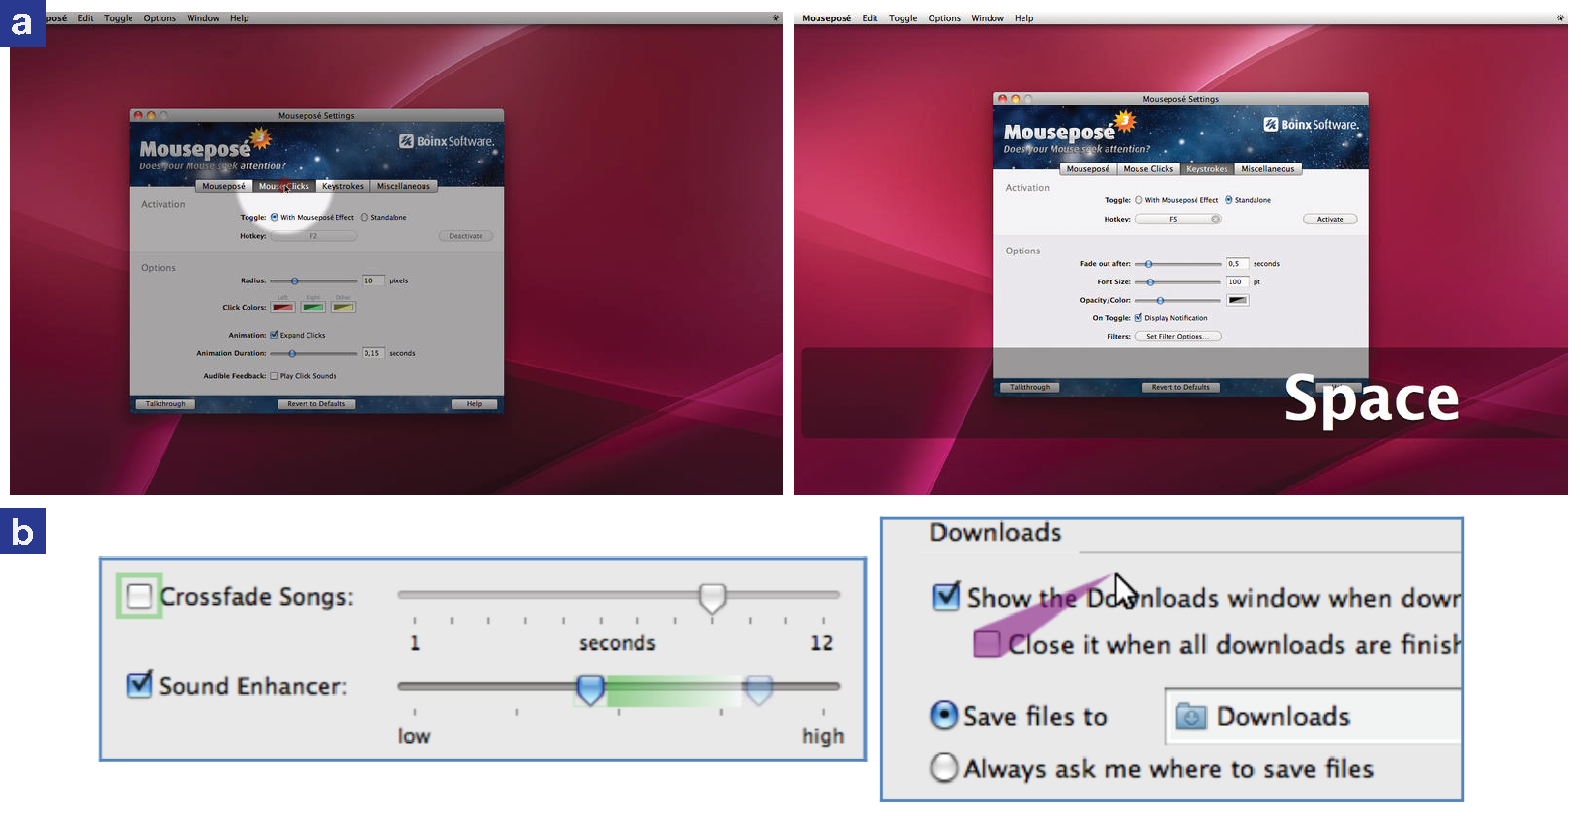
\includegraphics[width=0.7\textwidth]{\background/fig/realtime/realtime}
  \caption{Real-time visual enhancements on GUI applications: The top row shows how Mouseposé highlights a mouse cursor (left) and keyboard input (right); The bottom row presents Prefab~\cite{Dixon:2010fb}'s results of reverse engineering that identifies UI components and enables visualizations during author operations, such as afterglow~\cite{Baudisch:2006:PET:1166253.1166280} (left) and target-aware~\cite{Grossman:2005:BCE:1054972.1055012} (right) effects.}
  \label{fig:related_realtime}
\end{figure*}

\begin{figure*}[t!]
  \centering
  \includegraphics[width=0.6\textwidth]{\background/fig/software_viz/Nakamura_and_Igarashi}
  \includegraphics[width=\textwidth]{\background/fig/software_viz/Grabler}
  \caption{Example screenshots where mouse operations are automatically rendered, including (top) mouse move, drag, click, and wheel (a-d) by Nakamura and Igarashi~\cite{Nakamura:2008:ASV:1449715.1449721} and (bottom) application-specific operations (a-b), parameters (c-f), and manipulations (g-h) by Grabler \ea{}~\cite{Grabler:2009jj}.}
  \label{fig:related_events}
\end{figure*}

% in screenshots
The above methods enable real-time visualization of input events when operating an application, which are useful for following a video tutorial. However, they may not effectively present continuous actions, such as navigating a menu from the root to a sub-panel. For screenshot images in a static tutorial, visualizing input actions with motion arrows is a common technique to provide a sense of direction and start and end positions.
%
Researchers have investigated automatic approaches that capture and visualize these types of events in representative screenshots from author demonstrations. Nakamura and Igarashi~\cite{Nakamura:2008:ASV:1449715.1449721} proposed a capturing and rendering system independent to GUI applications. Their system logs mouse events of a software demo process, including mouse moving, dragging, and clicking. Operations are rendered as markers and arrows on screenshot images to present the linear event history (see Figure~\ref{fig:related_events} top).
%
Grabler \ea{}'s approach~\cite{Grabler:2009jj} further annotates a screenshot with bounding boxes and call-outs, which help learners identify parameters and options of software functionalities (see Figure~\ref{fig:related_events} bottom).

% summary
Our systems adopt some of these successful techniques to enhance visual instructions. By capturing event information at both input device and application levels, we visualize author operations based on different playback modes.
%
During \emph{video playback}, MixT shows mouse trails and actions, and DemoWiz overlays glyphs and arrows to guide viewers from the current input action to the next.
%
In a \emph{static}, step-by-step tutorial, MixT renders screenshot images with mouse visualizations, such as highlighting a drop-down menu.

% -------------------

\subsection{Workflow Capturing and Tutorials}
In addition to visualizing input events, it is important to present the entire workflow in a tutorial and provide concise instructions.
%
Grabler \ea{}'s system~\cite{Grabler:2009jj} generates a step-by-step tutorial from author demonstration (see Figure~\ref{fig:related_static}). Designed for instructing image manipulation tasks, it includes textual description from templates, such as \iquote{Select the \textbf{path tool} from the \textbf{toolbar} to \textbf{create and edit paths}.} The generated text and annotated images of operations are presented in a document to describe a workflow. Their work is available as a Photoshop plug-in\footnote{Adobe labs. Tutorial Builder. \url{http://labs.adobe.com/technologies/tutorialbuilder/}}.
% analyzes the application context, including facial features and outdoor scenes in manipulated images.
%
Such demonstration-based approaches have been applied to generate instructions for software that involves complicated manipulations or gestures, including 3D mesh construction~\cite{Denning:2011fy} and touch-based mobile applications~\cite{Wang:2014:EAC:2556288.2557407}.
%
Beyond logging input events during an author demonstration, researchers have shown that workflows and software content can be acquired using computer vision from analyzing desktop regions~\cite{Yeh:2009dh,Chang:2011vd} and existing screencast videos~\cite{Banovic:2012kd}.

\begin{figure*}[t!]
  \centering
  \includegraphics[width=0.8\textwidth]{\background/fig/related_static/grabler}
  \caption{Example static tutorial automatically generated by Grabler \ea{}'s system~\cite{Grabler:2009jj}.}
  \label{fig:related_static}
\end{figure*}

To compare effects of individual operations in a workflow, showing a list of ``before'' and ``after'' thumbnails, video clips, and event timeline can be effective \cite{Grossman:2010jz}, especially for image manipulation tasks (see Figure~\ref{fig:related_comparison} left).
%
When there are multiple workflows that create similar results, a union graph and side-by-side documents are useful for comparing operations~\cite{Kong:2012:DTR:2207676.2208549} (see Figure~\ref{fig:related_comparison} right).

\begin{figure*}[t!]
  \centering
  \includegraphics[width=0.4\textwidth]{\background/fig/software_viz/Grossman}
  \includegraphics[width=0.55\textwidth]{\background/fig/software_viz/Kong}
  \caption{Instructional systems that help learners compare effects and similar tutorials using (left) before and after images (a) and event timeline (b) by Grossman \ea{}~\cite{Grossman:2010jz} and (right) operation union graph by Kong \ea{}~\cite{Kong:2012:DTR:2207676.2208549}.}
  \label{fig:related_comparison}
\end{figure*}

% summary
These systems provided insights on 1) automatic generation methods of step-by-step tutorials and 2) workflow presentations serving for different purposes. Our MixT system is built based on the Photoshop plug-in (Tutorial Builder) to acquire a step-by-step document with text descriptions. We enhance the static tutorial format by embedding instructional video clips for each operation that can be interactively reviewed.

This paradigm opens a design space to create new tutorial formats that can be interactively reviewed. In recent years, researchers have shown that learners using responsive video tutorials~\cite{Nguyen:2015:MST:2702123.2702209} and learning-by-doing activities~\cite{Kwon:2016:CEO:2858036.2858101} performed better in following instructions than using static or video tutorials.

% -------------------

\subsection{In-Application Support}

The above methods introduce innovative ways for learners to review workflows and instructions. However, reviewing these materials is often separated from operating a software application. Learners might have to switch between the main application they are using and a separate set of instructions, which could introduce a gap of evaluation (\iquote{Am I doing this right as the instructions explain?}) and a gap of execution (\iquote{How do I perform the action that the instructions describe?}).
%
Researchers have proposed another approach to provide ``in-application'' assistance, often in real-time, in a specific application context.

There has been a considerable amount of research devoted to offering interactive help to support learners comprehend the functionalities while operating an application.
%
Crystal~\cite{Myers:2006:AWW:1124772.1124832} enables software users ask questions about ``why'' something did or did not occur in an application.
%
Video snippets can be embedded in application tooltips to explain specific functionalities~\cite{Grossman:2010wr}, which were shown to be seven times more effective than conventional tooltips for completing unfamiliar tasks.

Interactive, step-by-step instructions can be integrated in several forms:
%
To help software users identify specific UI components, tutorials can be shown via a translucent colored ``stencil,'' which visually directs user's attention in an application~\cite{Kelleher:2005:STD:1054972.1055047}.
%
By tracking user's current operations, tutorials can be embedded in an application to provide instant feedback such as a check-mark or a percentage match~\cite{Fernquist:2011:SRE:2047196.2047245}, automatically replayed to present the corresponding video instructions~\cite{Pongnumkul:2011ju}, or be shown as ambient help~\cite{Matejka:2011:AH:1978942.1979349}.
%
Instructions can be captured from demonstration as ``scripts'' for step-by-step navigation~\cite{Bergman:2005:DocWizards}. In-application controls~\cite{Lieberman:2014:SML:2557500.2557543} and game elements~\cite{Li:2014:CGM:2556288.2556954, Dontcheva:2014:CCL:2556288.2557217} can further engage users in learning.

As tutorials are built for a broader community with a set of authors and learners, content can be dynamically updated within a community based on user contribution~\cite{Lafreniere:2013ff,Matejka:2009:CCR:1622176.1622214, Bunt:2014:TPI:2556288.2557118}.

Our work focuses on authoring tools to create novel tutorial format designs, not the learning support. We see opportunities of combining our approaches with in-application guidance. For example, a video clip from a MixT tutorial can be automatically replayed when a system detects a slowdown of a learner's progress on a specific step. However, we do not claim contribution in this direction.

% These projects show how effective instructional representations can assist learners in learning or executing tasks. Our goal is to further study new formats that incorporate advantages of several formats of multimedia, including images, text, and videos, and in turn enhancing the learning experience for a variety of tasks.

% * define ``automatic''
% Note: MixT tutorials are automatically rendered from manual demonstration, not automatically generated.

% To provide real-time assistance, it is important to recognize the user activities during a task performance. Several domains have been widely studied, including software operations, scene recognition, and object tracking in a physical world.

% -------------------------------------------

\section{Instructions for Physical Activities}
\label{related_physical}

The above approaches of tracking a software demonstration open the door to enable interactive tutorials that can respond to user progress. However, understanding user behavior in the physical world, rather than in software, remains challenging.
%
How do technologies track humans and objects in a space to support real-time feedback? What are the available authoring techniques to generate instructions for physical tasks?
%
This section discusses the challenges from four perspectives, including tracking activities, authoring instructions, presenting guidance, and enabling interactive instruction following in a real world.

% -------------------

\subsection{Tracking Physical Activities}
To record activities and provide responsive feedback, a computer system needs to detect user operations and objects in real-time.
%
Computer vision techniques can automatically track specific physical targets shown in a video for interactive applications. These include three major categories:

\begin{itemize}
  \item \textbf{Tracking objects}. Common techniques include:
  1) Track specific \emph{colors} or visual features of pre-defined objects. Examples include tracking a fast-moving Ping-Pong ball for automatic camera control~\cite{Okumura:2011tr} or paper puppets for creating animation~\cite{Barnes:2008:VideoPuppetry}.
  %
  2) Track both \emph{colors and depths} of objects, which could obtain a better understanding of the objects' positions in a 3D world. The information can be useful for activities involved object manipulations, such as block or toy assembly tasks~\cite{Gupta2012DuploTrack,Wu:2016:ARI:2856400.2856416} and 3D puppet control~\cite{held20123d}.
  %
  3) Track \emph{motion-capture markers}. The most common method is to attach reflective markers to an object's surface. This enables accurate, responsive capturing, such as to record an animator's continuous movements~\cite{Dontcheva:2003:LAC:1201775.882285}.
  %
  \item \textbf{Tracking humans}. Targets include \emph{faces} (e.g., to show a close-up of a speaker during video conferencing~\cite{Ranjan:2010}, provide real-time camera control guidance when filming an interview video~\cite{Carter:2010}, and capture facial performances~\cite{Shi:2014:AAH:2661229.2661290,thies2016face}), \emph{hands} (e.g., to enable gestural control~\cite{taylor-siggraph2016} and camera control of a repair task~\cite{Ranjan:2008}), and \emph{user movements} (e.g., to provide augmented information~\cite{Wilson:2012fb,Anderson:2013:YEM:2501988.2502045}).
  %
  Motion-capture markers are often used to accurately track actors in professional filmmaking. However, since markers are visible in a camera view, visual effects (VFX) are necessary to post-process a video recording.
  %
  \item \textbf{A combination of the above}, such as reconstructing a 3D scene of a player throwing a basketball~\cite{dou-siggraph2016}.
\end{itemize}

Some of these vision-based systems require a high-speed camera~\cite{Okumura:2011tr} or a RGB-D camera~\cite{Gupta2012DuploTrack,Wu:2016:ARI:2856400.2856416,held20123d,Wilson:2012fb,Anderson:2013:YEM:2501988.2502045,dou-siggraph2016}, while some require users to wear reflective markers~\cite{Ranjan:2008}.
%
Other non-vision tracking methods rely on sensors attached to an object or human, including GPS sensor~\cite{HexoDrone} and radio frequency wireless signals~\cite{Nguyen:2016:ICR:2935620.2935632}. These are often used for tracking a moving target in a larger space, such as a flying drone.
%
Finally, if video content is difficult to be extracted, crowdsourcing algorithms have been introduced to structure step-by-step videos by online workers~\cite{Kim:2014:CSI:2611222.2556986}.

% summary
The detection mechanisms from these systems inspired us to design interactive systems that can react to authors' activities without requiring users to carry  a sensor. For examples, Kinectograph and DemoDraw track authors' body parts using a Kinect sensor that has been widely available to consumers.
%
However, tracking technique for high-level information, such as the \emph{intent} of a certain action, is yet lacking. Therefore, when automatic activity recognition is difficult, we include authors in a loop to annotate a task. DemoCut provides an annotation interface for describing DIY videos; DemoDraw provides a multi-modal interface to label continuous body movements.

% These methods usually require an expert defining heuristics of space regions or movement classifications ahead of time for the tracking program.

% -------------------

\subsection{Authoring Instructions for Real-World Tasks}

We identified two major approaches to create instructions for physical tasks: model-based and demonstration-based generation.
%
A \emph{model-based} system analyzes the structure of an object or a task and renders instructions.
%
The approaches by Feiner and Seligmann~\cite{feiner:1985:AEA:1299975.1300548,Seligmann:1991:AGI:127719.122732} considered communicative intent and rules of object manipulation to create 3D illustrations. Their automatically-generated results showed that actions such as snapping latches can be effectively expressed by motion arrows and a cutaway view.
%
By analyzing object geometry and other attributes, Agrawala \ea{}'s~\cite{agrawala2003designing} system automatically renders step-by-step assembly instructions, e.g., for furniture and toys (See Figure~\ref{fig:related_models} left).
%
Technical diagrams can also be generated, such as an exploded view that explains mechanical assembly parts~\cite{li2008automated} and motion illustrations that describe how individual parts are operated~\cite{mitra2010illustrating}. Parts are highlighted using colors, often labeled with text; Casual chain sequence of mechanical interaction can be shown as a list of highlighted figures, annotated with motion arrows (See Figure~\ref{fig:related_models} right).
%
Reversely, an existing technical document can be automatically analyzed and transfered into 3D animation by parsing the parts, orientation, and visual annotations~\cite{Mohr:2015:RTD:2702123.2702490}.

\begin{figure*}[t!]
  \centering
  \includegraphics[width=0.3\textwidth]{\background/fig/model_generation/furniture}
  \includegraphics[width=0.5\textwidth]{\background/fig/model_generation/chain}
  \caption{Example instructions automatically generated by Agrawala \ea~\cite{agrawala2003designing} (left) and Mitra \ea~\cite{mitra2010illustrating} (right) using model-based approaches.}
  \label{fig:related_models}
\end{figure*}

A \emph{demonstration-based} system records an author's physical demonstration of a workflow. The captured materials can be either automatically analyzed by the system or manually edited by an author to create instructions.
%
One approach is to employ templates to help users capture sequences of distinct shots (e.g., Snapguide\footnote{\url{http://snapguide.com/}}) or provide a limited set of operations to record specific moments (e.g., adding or removing a part in a block-assembly task~\cite{Ranjan:2007,Gupta2012DuploTrack}).
%
Another approach is to provide an interface to support authors capturing multimedia materials during or after a demonstration, such as using a head-mounted capturing device~\cite{carter2015authoring}. For certain tasks, new recording devices need to be specially designed, such as an integrated device that includes an IR camera to capture a knitting process~\cite{Rosner:2008:SAK:1409635.1409682} and a turntable to record the building process of a DIY project~\cite{Tseng:2015:SPT:2771839.2771869}.

% summary
In this dissertation, we support a wide variety of how-to tasks from craft to home repair and cooking where automatically tracking user activities is not yet completely possible. Since these domains often involve author creativity and personal styles, we opt for the demonstration-based approach.
%
DemoCut, Kinectograph, and DemoWiz each allows authors to perform a physical demonstration in front of a camera, while semi-automatically capturing the activities.

% -------------------

\begin{figure*}[t!]
  \centering
  \includegraphics[width=0.4\textwidth]{\background/fig/ar/authoring}
  \includegraphics[width=0.41\textwidth]{\background/fig/ar/following}
  \caption{TeleAdvisor~\cite{Gurevich:2012ko} provides an authoring interface (left) for an instructor to guide a remote worker through a repair task (right).}
  \label{fig:related_teleadvisor}
\end{figure*}

\begin{figure*}[t!]
  \centering
  \includegraphics[width=0.55\textwidth]{\background/fig/ar/technical_document}
  \caption{Work by Mohr \ea{}~\cite{Mohr:2015:RTD:2702123.2702490} automatically analyzes a technical document and augments a machine with AR animation in 3D.}
  \label{fig:related_ar_annotation}
\end{figure*}

\subsection{Presenting Guidance}
To help learners perceive instructions for physical tasks, we discuss how guidance can be displayed in a 3D world. There are four main approaches to present real-time guidance.

First, rich information can be shown via an \emph{external display} placed next to the work area. Several applications adopt this method, including cooking~\cite{Uriu:2012:PRM:2207676.2207695} and block assembly tasks~\cite{Gupta2012DuploTrack,Wu:2016:ARI:2856400.2856416}. However, a learner may often switch his or her attention between the task and the instructions. To better blend the information into activities, Knibbe~\ea{} designed a display-embedded table as a physical workspace that monitors, records, and assists users~\cite{Knibbe:2015:SMI:2817721.2817741}. In this way, workers can review the information on the desktop while making a project.

Second, information can be \emph{overlaid on top of the work area} through a projector. Examples include supporting remote repair tasks~\cite{Gurevich:2012ko} (see Figure~\ref{fig:related_teleadvisor} right), assembly tasks~\cite{Kirk:2006:CRG:1124772.1124951}, cooking~\cite{Ju:2001:CIC:634067.634227}, and piano learning~\cite{Xiao:2016:IEI:2858036.2858577}.
%
For tasks such as dance movements, guidance can be shown on an augmented mirror that learners constantly focus on~\cite{Anderson:2013:YEM:2501988.2502045}.
%
This method can effectively present instructions at a location that can be viewed by a learner during a task. However, this often requires a specific indoor environment setup and a calibrated projector, which is not scalable.

Third, information can be \emph{augmented through a head-mounted display or a mobile phone} accessed and viewed by individuals. Researchers have shown AR applications that provide visual highlights for machine maintenance~\cite{Henderson:2011ff,Mohr:2015:RTD:2702123.2702490} (see Figure~\ref{fig:related_ar_annotation}), enable interactive touring in a city~\cite{Feiner1997}, explain product functionalities~\cite{MagicLens}, and present dynamic UI or information based on head orientation~\cite{Zhang:2014:HHO:2659766.2659773}.
%
Compared to the previous approach that projects information onto a public space, this method allows learners to access information individually. Multiple users can interact with an augmented system at the same time. However, learners have to wear or hold a device, which might limit their mobility while performing a task.

Last, for specific tasks, information can be conveyed \emph{directly via target objects}. Haptic feedback has shown to be useful to help learners capture guidance while focusing on the physical tasks, such as for sculpturing~\cite{Zoran:2013:FFD:2470654.2481361,Agrawal:2015:PPS:2807442.2807505}, building multi-material assemblies~\cite{Schoop:2016:DSS:2851581.2892429}, and learning Frisbee~\cite{Solomon:2014:UTI:2540930.2540965}. Visual cues such as LED patterns shown on a device can help direct user's attention~\cite{Solomon:2014:UTI:2540930.2540965,Vasey:2016:HHR:2897839.2927404}.
%
This approach is task-specific and can be difficult to generalize to other task domains.

\subsection{Providing Interactive Guidance}
% \subsubTitleBold{Responding to Learners' Progress}
Finally, we discuss how assistive technologies track a learning process and support interactive guidance. Providing responsive feedback requires an understanding of learners' activities. For specific tasks such as block assembly~\cite{Gupta2012DuploTrack,Wu:2016:ARI:2856400.2856416} and dancing~\cite{Anderson:2013:YEM:2501988.2502045}, learners' progress can be accurately tracked in 3D. This enables a tutorial system to provide real-time information about the current learner state, e.g., where to place the next block to the current model or suggested adjustment on a dance pose.
%
However, as we discuss earlier, tracking activities at the instruction level for real-world tasks is still lacking. Therefore, the majority of the systems provided user interfaces for learners to navigate instructions.
%
For a pair learning scenario, a remote instructor can manually provide instructional input based on the learner's progress that he or she sees, such as highlighting a component for remote repair tasks~\cite{Gurevich:2012ko,Kirk:2006:CRG:1124772.1124951} (see Figure~\ref{fig:related_teleadvisor} left).

Our work focuses on designing tools for tutorial authors to create instructions from demonstrating a task. DemoCut is designed for authoring instructions after the capture time. Kinectograph provides an control interface on a Tablet device for authors to carry and place in a space. DemoDraw's demonstration interface is similar to Anderson \ea{}'s~\cite{Anderson:2013:YEM:2501988.2502045} augmented mirror. But instead of overlaying instructions, we present a real-time rendering view of an author's movements via an external display placed in front of the user. We have not investigated tools for learners to follow a task.

% -------------------------------------------

\section{Working with Videos}
\label{related_videos}

Research in video understanding has introduced new ways to work with videos, including capturing, editing, and navigating. How do authoring tools help users record, organize, and edit necessary materials? What are the interaction techniques of reviewing one or multiple videos? In this section, we review these topics briefly.

% -------------------

\subsection{Capturing}
Tool supports at the capturing phase include:

\subsubTitleBold{Filming Suggestion}
Several research systems guide users at capture time to yield higher-quality videos. Real-time suggestions include framing of the subject or camera view (e.g., NudgeCam for interview videos~\cite{Carter:2010}) and actor's performance~\cite{Heer:2004ba,Davis:2003cu}. Shot suggestions can also be bootstrapped through user dialogs~\cite{Adams:2005}.
%
Patterns from expert storytellers and commonsense reasoning can recommend novice authors to capture materials and develop a story structure~\cite{Barry:2003:MCC:957013.957152,Kim:2015:MSN:2702123.2702507}.

\subsubTitleBold{Camera Control}
Viewpoints of stationary cameras can be automatically decided based on heuristics at record time to trace an actor, an area, or an object~\cite{Ranjan:2008,Okumura:2011tr}.
%
In recent years, quadrotor cameras enable a wide range of trajectories to capture a subject from different viewing angles. Roberts and Hanrahan~\cite{Roberts:2016:GDF:2897824.2925980} proposed an authoring tool for authors to plan and preview a camera trajectory. When being filmed, 3D gestures allow a person to control a quadrotor camera at the scene~\cite{Cauchard:2015:DME:2750858.2805823,Pfeil:2013:EGM:2449396.2449429}.

% summary
We proposed Kinectograph prior to these systems of quadrotor camera control. A recent commercial system has included a similar feature to track a moving user~\cite{HexoDrone}, which is based on GPS location instead of specific body parts.

% -------------------

\subsection{Editing}
Tool supports for video composition and editing include:

\subsubTitleBold{Annotation}
Researchers have investigated how to provide interactions that enable efficient, fluid annotation or labeling of video data. Examples include the EVA system~\cite{Mackay:1989} that encouraged authors to annotate materials at capture time. More recent interfaces leverage pen input (e.g., VideoTater~\cite{Diakopoulos:2006vt}) and touch or gestural input~\cite{Sarkar:2016:SCC:2858036.2858199}.

\subsubTitleBold{Story Composition}
When working with a repository of video clips, it can be challenging to compose a compelling story. Several new interaction techniques have been proposed:
%
A storyline can be created non-linearly based on relevant characters, emotions, and themes of the current edited clips~\cite{Shen:2009:WNE:1518701.1518825}.
%
Tangible controllers with a specialized table interface enable collaborative, non-linear editing~\cite{Bartindale:2012:STS:2207676.2207700,Bartindale:2016:TSS:2818048.2819929}.
%
Live authoring at capture time with a Tablet device allows an author to quickly organize clips and apply editing decisions~\cite{Freeman:2014:LLA:2611105.2557304}.

\subsubTitleBold{Computer-Powered Editing}
Frame-based editing of video is very time-intensive, as it forces users to operate at a very low level of detail. Editors can leverage \emph{metadata}, such as shot boundaries~\cite{Casares:2002dx} and transcripts~\cite{Berthouzoz:2012} that help users place cuts and transitions. This gives users higher-level editing operations at the shot level rather than the frame level.
%
Techniques of \emph{computer vision} and \emph{speech analysis} can automate certain visual effects, such as creating cinemagraphs~\cite{Bai:2012, Joshi:2012}, automatically-edited lecture videos~\cite{Heck:2007}, zoomable tapestries~\cite{Barnes:2010} and synopses~\cite{Pritch:2009vl}, or stabilizing shaky amateur videos~\cite{Liu:2011}.
%
Edits can take place during recording, such as switching to a close-up view of a person who is speaking~\cite{Ranjan:2010}.
%
When material can be reviewed in 3D such as character animation, camera angles can be optimized to render a new video by analyzing the actor data~\cite{assa2005action,assa2008motion}.
%
Finally, when video analysis is a matter of subjective taste, identifying salient frames or highlights can be outsourced to crowd workers~\cite{Bernstein:2011uj,Tang:2012:ECS:2207676.2208622}.

% summary
MixT, DemoCut, Kinectograph, and DemoDraw also use vision techniques for automatic editing. They differ from previous approaches in its focus on two particular application domains -- software and physical demonstration videos.
%
By focusing on a specific domain, MixT and DemoCut can make assumptions about the structure of the input and output video, such as the fact that there is a linear set of steps, and offer an interface and algorithms that make it easier to create high quality how-to videos.
%
Kinectograph makes editing decisions (e.g., pan-and-tilt, zooming) based on actor's body location for instructional videos.
%
DemoDraw includes a multi-modal interface where authors can annotate a motion recording using speech while physically performing movements.

% visual enhancement~\cite{Santosa:2013:DST:2470654.2466148}

% -------------------

\subsection{Navigating}
% Tool supports for video navigation include:
Automatic video control can follow user actions or preferences, such as segment playback when operating software applications~\cite{Pongnumkul:2011ju} or playback speed control~\cite{Cheng:2009:SUV:1518701.1518823}.
%
Videos can be navigated at the content level beyond a linear timeline, such as visualizing subject movements in a storyboard design~\cite{goldman2006schematic} or a continuous image mosaic~\cite{Teodosio:2005:SS:1047936.1047940} and enabling direct manipulation of a target in 2D~\cite{Dragicevic:2008:VBD:1357054.1357096,Goldman:2008:VOA:1449715.1449719,Karrer:2008:DDM:1357054.1357097} or 3D~\cite{Nguyen:2013:DMV:2470654.2466150}.
%
These techniques help viewers understand content flow and playback videos, and have been applied to screencast videos~\cite{Denoue:2013:RDM:2451176.2451190,Nguyen:2015:MST:2702123.2702209}.
%
To further navigate a long video or a set of videos, a canvas showing video tiles and timeline was shown to be 36\% faster than a conventional list view~\cite{Al-Hajri:2014:VPH:2611105.2557106}. A video digest is effective in browsing and skimming video content~\cite{Pavel:2014:VDB:2642918.2647400}.
% Lecture videos~\cite{Tang:2006:DIU:1111449.1111523},

These novel forms of video navigation inspired us to explore new visual and playback designs for revealing the video content.
%
MixT supports per-step video navigation embedded in a static tutorial.
%
DemoWiz augments a screencast video with novel visualization for following the content.
%
DemoDraw renders a series of human movements as concise motion illustrations.

% In contrast to these systems, we do not require the author to manipulate the camera or system during capture. Many leisure activities, such as home repair or cooking, require use of both hands or involve getting one's hands dirty, so camera manipulation is not possible. We use vision techniques for automatic recording and editing. It differs from previous approaches in its focus on particular application domains -- software and physical demonstrations. By focusing on specific domains, we can make assumptions about the structure of the input and output video, such as the fact that there is a linear set of steps or movements, and offer user interfaces and algorithms that make it easier to create high quality instructions.

%!TEX root = ../thesis.tex

\section{Principles and Methods}
% Motion Illustration
% \bjoern{this section is too long for the work it does - more than page! Shorten.}
% \dan{I did some trimming, now a few lines more than a column without comments (not counting figure).}
% \dan{The main takeways after reading this section should be: 1) the style of illustration our system supports matches what people actually need; 2) current practices are slow and/or require specialized skills; 3) automating the first part of the process is most important: generating (and experimenting with) keyframe illustrations with motion annotations from real time demonstrations. } \bjoern{Yes!}

To understand motion illustration design and production, we surveyed related literature, studied found examples, and interviewed individuals who create such illustrations.

\subsection{Design Principles}
%to evaluate five general methods
Cutting~\cite{cutting_representing_2002} argues that superimposing vector-like lines on an image satisfies four important criteria: it evokes a feeling of motion, the object undergoing motion is clearly represented, the direction of motion is clear, and the magnitude of motion is conveyed with reasonable precision. To complement this metaphoric representation, Cutting also argues for the more literal method of multiple stroboscopic images, which satisfies all criteria except clear motion direction. McCloud~\cite{mccloud_understanding_1994} provides further arguments and examples for using these methods in the field of comic illustration, and notes communication benefits when they are combined.

To examine how professional illustrators use motion lines and stroboscopic images, we gathered examples from sources like user manuals, gesture-based games, safety guides, % (e.g., for airplane safety or weight training),
illustration compendia (e.g.,~\cite{mijksenaar1999open}) and how-to books (e.g.,~\cite{greenberg2012sketching}).
%
We found Cutting's notion of vector-like lines are almost always rendered with an arrowhead % with of a clear head at the end of a line tracing the motion path.
in a variety of styles (heads, weights, colors) with strokes typically two-dimensional, smooth, and offset to avoid occluding the object.
Stroboscopic images can be overlapping or spatially distributed, and change in transparency or shading to convey time.
The most common style for depicting the object undergoing motion is a simplified black-and-white contour drawing, but filled silhouettes and flat-shaded colour can also be found -- using full color photographic detail is rare.
%
By carefully removing extraneous details, such techniques help readers focus on only the salient, abstract information.
% \bjoern{Add WHY - omit extraneous details to focus on salient features.}

% These methods can be used with the object undergoing motion rendered as a full color photo or as a stylized illustration with reduced detail. \dan{One or two sentence giving benefits of using illustrations over photos that adds more detail to the general argument in the introduction [references in Pat Hanrahan's lecture slides, maybe Buxton's sketching book ] } Early in the 90s, Dooley and Cohen designed a method to generate line illustrations from geometric model \cite{Dooley:1990:AIG:91394.91422, Dooley:1990:AIG:91385.91422}. This...

% http://vis.berkeley.edu/courses/cs294-10-fa13/wiki/index.php/Conveying_Shape:_Lines#readings

% NOTES

% - -

% Cutting (2002)
% (this article is amazing)

% 4 criteria for
% evocativeness: a feeling of movement
% clarity: can the object undergoing motion be easily identified
% direction: where is the object moving?
% precision: what is the magnitude of the motion?

% 5 general techniques to convey motion:
% dynamic balance: choose a pose to convey sense of movement (questionable direction, poor precision)
% affine shear: leaning into the direction of movement (evocative and somewhat clear, Cutting says direction is good(?))
%  motion blur (only evocative)
% stroboscopic images: “Motion as time discretely sampled” (poor direction (?) )
% arrows (action lines, speed lines), a more literal representation of the motion vector … Cutting says this is best: (evocative, clear, direction, precise)

% literal representations of motion (strobing, motion blur) and metaphorical (arrows, action lines)

% - -

% McCloud (1993)
% (need to read more)

% talks about benefits of combining stroboscopic and action-line (headless arrows)

% - -

% OpenHere

% Interesting history of the arrow (p19) -- it's a somewhat recent convention.

% kind of off-the-cuff description of different arrow and lines types on p102 (e.g. dotted lines indicate stages of movement)

% many techniques for visual instructions come form cartoons (e.g. lines for movement)

% - -

% Pat Hanrahan’s lecture slides (provides references to justify using illustration over photos ssaying  ``Illustrations often better than photographs, they enhance important features and emphasize unimportant detail''

% - -

% Buxton, Sketching Interaction

% (didn’t find anything relevant beyond comments about arrows being good for conveying motion … our work isn't really about sketching, we're illustrating.)


\subsection{Interviews: Methods Used In the HCI Community}
% https://docs.google.com/document/d/1TisNlsFUYQ3a-BuqryRv8qmyp3La-qLj-j3hN4PyVS8/edit
% \bjoern{The challenge here is that HCI researchers with Illustrator chops are MUCH closer to experienced designers than the general population. So using HCI authors to make an argument about ``non-designers'' is problematic. I took it out.}
% The examples we gathered above are produced by professional illustrators, but many other people create motion illustrations as part of their work --
% A central goal of our system is to empower individuals to rapidly create professional-quality motion illustrations.
To understand current creation methods, we conducted video interviews with six Human-Computer Interaction researchers with experience creating motion illustrations.
%
Conveying movement for interaction is common in HCI publications. We found 100 motion illustrations in 58 recent papers.

%We conducted interviews with 6 researchers with experience creating motion illustrations.
% We surveyed papers published between years 2005 to 2014 that contained motion illustrations in venues such as CHI, UIST, and MobileHCI -- we found whole-body motions, such as play in an interactive room and large display interactions; and  hand motions, such as smartphone interactions. We conducted video interviews with six authors of such papers about their process.

% and found
%100 motion illustration figures in 58 papers. From a pool of authors who created illustrations in two or more of these papers, we invited 6 to share their experiences (aged 25-43, all males: 3 professors, 2 industry researchers, 1 graduate student).
%Two participants had some design or art background.
%
%Interviews were conducted by video conference for one hour. The discussion focused on the creation process for 2 to 4 figures which we selected from the interviewee's papers. Selected figures for two interviewees were whole-body motions, such as game play in a room space and large display interaction; figures for the rest were hand motions, such as smartphone or hand-held device interaction.

\subsubTitleBold{Findings}
% in 3 categories: tools and creation process, motivations, and struggles
% Several authors emphasized the importance of concision and focus: they introduced important concepts via illustrations with unnecessary details excluded, like faces, clothing, and backgrounds. Establishing a consistent visual style was important to reuse graphic elements. %, especially for operating mobile devices.
%
All interviewees used a similar methodology to create motion illustrations: they took still photographs of people performing actions, traced outlines using Adobe Photoshop (4/6) or Illustrator (2/6), then added graphic annotations to convey motion. %One interviewee with design expertise sometimes drew illustrations from scratch.
%All interviewees mentioned the importance of iterating illustrations. Often preliminary versions were created for an early draft and refined later.
% 4 of the 6 interviewees used Photoshop, while 2 used Illustrator; 3 solely used a mouse while 3 used a stylus as a main input device.
%
All mentioned that it was time-consuming to set up scenes and poses, take and trace photos, then add details like arrow placement while maintaining a consistent style. Typical creation times were estimated between 10 minutes to a few hours.
They also noted how difficult it was to make adjustments: changing the pose or viewpoint essentially meant starting over again with new source photos and re-tracing.
Yet, identifying the best pose and viewpoint ahead of time is difficult and it often took several iterations to yield an illustration suitable for publication.
% \dan{I added the last sentence, Peggy please confirm that aligns with what you heard in the interviews ... I know at least I said that ;)}

\begin{figure}[t]
  \centering
  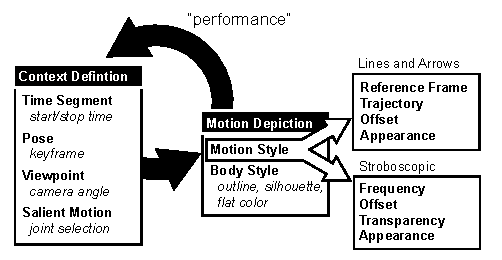
\includegraphics[width=\columnwidth]{\demodraw/fig/designdimensions}
  \caption{Canonical authoring workflow consisting of a Context Definition task then a Motion Depiction task. Design decisions associated with a task shown in bold with design parameters in italics.}
  \label{fig:designspace}
\end{figure}

\subsection{Design Space Goals and Workflow}

Based on the above, we derive a canonical workflow to motivate the central design goal for our system.
Authors face two primary illustration tasks (Figure~\ref{fig:designspace}):
\textit{defining the context} for portraying motion like the view of the body and salient aspects of motion;
and \textit{exploring a style of motion depiction} by choosing styles like lines-and-arrows or stroboscopic, then adjusting related style parameters.
These tasks and the underlying design parameters are highly interdependent, so authoring motion illustrations is necessarily an iterative process.
This means that changes to one task parameter often leads to re-evaluating and changing the other.
The problem with current methods, is that context is mostly ``performed'' using a time-consuming process of taking photos and manually tracing them.
%
Therefore, the central design goal of our system is to make context definition  low effort and iterative by using interactive demonstrations for automated context definition.

% enable low-effort iteration within, and between, the three identified tasks.

% %When creating illustrations, there are two primary tasks: 1) \textit{selecting the body context} and 2) body and motion \textit{depiction} (Figure~\ref{fig:designspace}).
% %\dan{I think ``context'' and ``depiction'' capture what people do, but maybe there are better terms.} \bjoern{yeah i don't understand them.}
% Performance capture involves recording suitable primary material to analyze and visualize. Identifying salient aspects
% %Selecting the body context
% involves segmenting a motion into steps, selecting key poses,
% %adjusting the camera angle to optimize the depiction of the pose and motion annotations,
% and identifying joints as salient motion for annotation. Depiction involves selecting a body visualization style, picking a motion visualization style (lines-and-arrows or stroboscopic), and adjusting many specific motion style parameters.
% These design parameters are all highly interdependent.
% %which is why the sequential and manual creation processes used by our interviewees is so time-consuming.


%Since current methods for the context setting task are time-consuming and inflexible, our system places extra focus on enabling rapid iteration.

Designing a system to capture interactive demonstrations of \textit{any} body movement also poses an input challenge.
Since  body movements form the demonstration itself, also issuing application commands with a body gesture introduces ambiguity.
Using a hand held device, touch screen, or any conventional input is not ideal since performing requires open space and full freedom of movement.
For these reasons, we use a multi-modal voice and gesture interaction style traced back to Bolt's Put-That-There~\cite{Bolt:1980:PutThatThere}. Like Bolt, we use voice for commands like \iquote{start} and \iquote{stop} with body movements providing command parameters in the form of the recorded demonstration, and for setting parameter context with utterances like \iquote{one, two, three, four} to label step-by-step segments.

%\peggy{We did not mention the reason we chose speech/voice for input. I briefly mentioned it in Pipeline in one sentence, but do we want to add a subsection here or mention in Introduction?}
%\dan{I added the paragraph above.}

% In addition, using manual techniques like photography or general purpose drawing tools like Adobe Illustrator means task parameters are highly under-constrained. This means the burden of upholding good design is placed on the non-expert user.
% A second goal of our system is to constrain the parameter space so that visualization principles are maintained.
% \dan{not sure if we do this second goal well}


% Lines: We may want to mention smoothing here? Several participants thought our system nicely smoothed the curves/arc (but should also straighten lines) even if their demo or Kinect mocap was not perfect.
% - Arrows: Double-headed arrows indicate repetition. DemoDraw does not adjust this automatically, but authors can manually change it to assign the intention.
% - Stroboscopic: also transparency? (had some meaning beyond appearance)
% - Sequencing: 1) DemoDraw generates the step-by-step diagrams based on motion segments, but also 2) Stroboscopic effect indicates the sequence of 2+ poses.

% \bjoern{Somewhere in the prior section or following section: Describe the design space of decisions one has to make to design an effective illustration. And argue that this is necessarily an iterative process where changes to one dimension may lead the designer to re-evaluate and change other dimensions. This is not possible with the current manual workflow starting with photos - authors are locked into a linear pipeline.}

% provide parameters, flexibility, direct manipulation, iterative design process



%!TEX root = ../thesis.tex

\subsection{Design Implications}

Based on our analysis of existing video tutorials and interviews with
tutorial authors, we identified a few key aspects of the tutorial creation
process that have important design implications for DIY video
editing systems.

\subsubsection{Working with single take, single camera footage.}
%
Most amateur authors record demonstrations in a single take with a
a single camera. As a result, the captured footage often includes
mistakes and long, repetitive actions.

\subsubsection{Making concise videos.}
%
The most important design principle for creating effective DIY videos
is to make them concise without sacrificing clarity. To this end,
authors remove/condense unnecessary or repetitive actions so that the
resulting video only contains salient footage.

\subsubsection{Retiming audio and video tracks separately.}
%
One common technique for speeding up a video involves breaking the
synchronization between the audio and video tracks so that they can be retimed
separately. In cases where the narration refers to
specific visual events, the tracks should remain aligned.

\subsubsection{Emphasizing important information.}
%
Most effective DIY videos include titles, annotations and/or closeup
views to emphasize relevant information and highlight key details.

\subsubsection{Focusing on high-level editing decisions.}
% Editing captured footage is a difficult and time-consuming task.
Amateur users often struggle with low-level manipulation of cut points and timing in general-purpose video editors: A system should reduce the editing efforts and enable authors to focus on making simple choices for the final production.

We next describe how these considerations informed the design of DemoCut.

%!TEX root = ../thesis.tex
\section{Authoring}
To enable amateur users to produce effective video tutorials, the DemoCut video authoring system semi-automatically edits a long, single take recording into meaningful steps.
Early testing revealed that users find it easier to locate specific {\em moments} in the video than to mark or edit {\em segments}. Therefore, our Annotation Interface asks users to mark important moments.
%
DemoCut combines the user annotations with audio and video analysis to automatically generate a segmented video with editing suggestions:
%
It removes or condenses unnecessary/repetitive actions and enables flexible synchronization between audio and video tracks.
Titles, visual annotations and closeup views are applied to enhance the content.
%
Users can review and revise these decisions in the DemoCut Editing Interface.
This section reviews DemoCut from the user's perspective (Figure~\ref{fig:block-diagram}). The following section will describe our video analysis pipeline.

\begin{figure}[t]
  \centering
  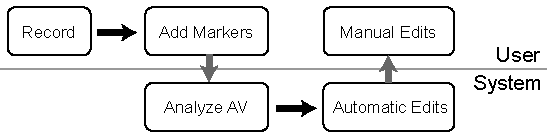
\includegraphics[width=1.0\columnwidth]{\democut/fig/block-diagram}
  \caption{DemoCut users first mark their recorded video in the Annotation Interface. DemoCut then segments their recording and suggests video edits, which users can change in the Editing Interface.}
  \label{fig:block-diagram}
  \vspace{-0.15in}
\end{figure}

\subsection{Annotating the Video}
The purpose of the DemoCut Annotation UI is to collect high-level information that is difficult to extract automatically but useful in determining how to edit the video.
We rely on users to distinguish important from unimportant actions and successful steps from mistakes.
The user scrubs through the captured footage and adds markers for distinct moments, such as the instant when he cuts a sheet of paper (Figure~\ref{fig:ui}A). DemoCut offers five types of markers for annotating a video:
\begin{itemize}
  \setlength{\itemsep}{0pt}
  \item \emph{Step}: indicates the start of a major part of the task
  \item \emph{Action}: marks important moments
  \item \emph{Closeup}: indicates moments where the action is happening in a small region of the video frame, e.g., for a detailed action such as fastening a small screw. %User can specify a zoom region.
  \item \emph{Supply}: indicates a tool or material used in the task
  \item \emph{Cut-out}: indicates moments of the video that should be removed due to occlusion or a mistake in the performance.
\end{itemize}
This set of markers was derived from our observations of the structure of effective tutorial videos: actions are treated separately from supplies; zooming can direct the viewer's attention to a small area of the frame; and step divisions are used to divide actions into meaningful groups. Rather than specify start and end frames, users can place a marker on any frame of an important moment.
%Each genre of video will likely have a different set of semantic markers.

Users can add descriptions to markers (Figure~\ref{fig:ui}B). These descriptions serve a dual purpose: they are used to generate automatic subtitles, and they are also shown as segment names in the Editing Interface to facilitate navigation. Users can also add visual highlights such as boxes and arrows to any marker.
%The collected meta-data is then used for later analysis.

\subsection{Automatic Video Editing}
Based on the user's markers, DemoCut automatically segments the raw footage and applies editing effects.
%To automatically segment the video, DemoCut uses two types of analysis. First, it looks for changes in the video around markers using frame differencing. Second, it detects narration through audio analysis. It combines the video and audio analysis to select appropriate editing effects from two classes: temporal effects and visual effects. The user can change effects selected by the system in the Editing Interface.

\subsubsection{Temporal Effects}
We designed four temporal effects to shorten a video. In addition to skipping a segment or leaving it unchanged, we consider the synchronization between the audio and video tracks: People are sensitive to changes in speech playback speed, but video can often be accelerated without loss of clarity. Therefore,
%-- especially of idle time, slow or repetitive movement --
%\bh{We know this intuitively, would be nice to find a reference}.
our temporal effects accelerate or contract video but keep audio at normal speed.

{\em Fast motion (with merged audio)}: When a segment includes several sections of narration with intermediate pauses, DemoCut removes the pauses and concatenates the audio segments. Then it speeds up the video so the total video length corresponds to the length of the concatenated audio (Figure \ref{fig:fastmotion}A). This effect is appropriate if tight synchronization between audio and video is not required. For example, an author may describe general strategies for choosing supplies while measuring paper -- here audio and video are independent of each other. In this case, DemoCut will accelerate the video %of salad mixing
to fit the length of the author's remarks.
%This is our default effect.

{\em Leap frog (with synchronized audio)}: If synchronization between audio and video is necessary, this effect plays video and audio at normal speed during active audio segments, and skips video in the interstitial segments (Figure \ref{fig:fastmotion}B).
Synchronization is important if the author's face is in the shot (so lip movement and audio match), if actions produce distinct sounds (like cutting paper), or if the narration refers specifically to actions, e.g., when pointing at an object and describing its properties.
Since DemoCut cannot automatically decide whether synchronization is necessary,
% and it tries to aggressively shorten the video,
it applies the Fast Motion effect by default but offers users control to change that effect.

{\em Skip:} Depending on the length of the removed segment, DemoCut either applies a fade through black (for segments up to 15 seconds); or a fade to a title that indicates how much time has passed (e.g., ``2 minutes later'').

If these temporal effects are not appropriate, DemoCut plays the audio and video at the captured rate. We call this the {\em Normal} effect.

\subsubsection{Visual Effects}
In addition to manipulating time, DemoCut offers three visual effects to structure the video and to provide emphasis. These visuals appear for the duration of the segment DemoCut derived from the user's marker:

{\em Subtitles}: Text entered by the user in the marking phase is converted into automatic subtitles with two levels -- a step heading that remains on screen for all segments within a step (e.g., ``Wrapping the present''); and a subheading from individual event markers (e.g., ``Sharpen creases'').

{\em Automatic zoom}: When users create closeup markers, they also specify a rectangular region of interest. DemoCut automatically crops and enlarges this region of the segment.

{\em Visual annotation}: DemoCut overlays visual box or arrow annotation specified by the user in the marking stage.

%\begin{itemize}
%  \setlength{\itemsep}{0pt}
%  \item \emph{Fast motion with merged audio}: when a shot includes several audio segments % (EXAMPLE: Salad dressing 1:32-)
%  \item \emph{Autocut with synchronized audio}: Alternative option
%  \item \emph{Fast motion}: when a non-closeup shot contains neither movement nor long narration % (EXAMPLE: Salad dressing 11:49-)
%  \item \emph{Skip}: cut-out shots marked by user % (EXAMPLE: Salad dressing 6:30-, Front light 2:56-, 3:22-)
%  \item \emph{Normal}: when there is movement % (EXAMPLE: Front light 3:17-)
  % \item \pc{\emph{Freeze}: if a closeup is too short} - ? % (EXAMPLE: Salad dressing 10:38-)
%\end{itemize}

\begin{figure}[t]
  \centering
\includegraphics[width=1.0\columnwidth]{\democut/fig/fastmotion}
  \caption{DemoCut accelerates playback of video with intermittent audio narration through Fast Motion (A) and Leap Frogging (B).}
  \label{fig:fastmotion}
  \vspace{-0.1in}
\end{figure}

\vfill
\subsection{Reviewing and Editing}
Since our automatic video and audio segmentation has a limited understanding of the video, it is likely that some editing decisions will be incorrect. For example, DemoCut's algorithms have no way of inferring whether audio-video synchronization will or will not be required in a given segment. In addition, automatic analysis may also lead to errors: if the narration is not correctly segmented, speech can be cut off mid-sentence. DemoCut's editor gives authors the opportunity to review and revise all editing decisions.

In the Editing Interface, the video is visualized as a set of segments (Figure \ref{fig:ui}E) flowing from top to bottom on the right side of the main video view (Figure \ref{fig:ui}C). There is no traditional timeline for two reasons: first, editing operations only apply to detected segments (we consciously prevent users from applying frame-level edits to keep with the goal of a semantic editor); second, because segments may come with labels entered by the user, a vertical layout makes it easier to read labels. Users can navigate to any segment by clicking on its thumbnail. Once selected, they can change which effect should be applied to a given segment (Figure \ref{fig:ui}D). Users can also modify any visual effects, to edit subtitles, resize the cropped region, or add/delete highlights. When satisfied with their choices, users can export a continuous video suitable for online video sharing platforms.

%\subsection{Tutorial Outputs Formats}
%\bh{Cut, shorten or merge with previous?}
%Finally, DemoCut produces the edited video in three formats:
%\begin{itemize}
%  \setlength{\itemsep}{0pt}
%  \item \emph{Video only}: a complete video clip with subtitles and effects for video %sharing platforms.
%  \item \emph{Indexed video}: a video player with markers below the timeline, similar to %the DemoCut Annotation UI. Viewers can navigate to a specific instruction via the marker %buttons.
%  \item \emph{Step-by-step instructions}: a series of mixed-media instructions on a web %page. Researchers identified how ... \cite{Chi:2012:MAG:2380116.2380130}.
%\end{itemize}

% \bh{say something about exporting in different formats?} \pc{move this subsection back from future work}

%Answer: why not provide visual sense of time

%visualize timeline: modified from timeline.js \cite{Cazenave:2011dg}
%\bh{I don't think you want to describe this as a UI for the author - this is a debugging tool for us and a %tool to explain the analysis through figure in the next section}.

%!TEX root = ../thesis.tex
\section{Automatic Effect Decision Pipeline}
DemoCut performs several automated steps to convert the user-annotated
input recording into an edited video tutorial. First, the system segments the recording into regions around user-specified markers. This segmentation considers both the
similarity of video frames around each marker and the presence of
narration in the audio track in order to determine the appropriate
segment boundaries (Figure~\ref{fig:democut_pipeline}). DemoCut then automatically applies an temporal and a visual effect to
each segment based on the type of the corresponding user marker and
the properties of the audio/video content in the segment. The rest of
this section describes these steps in detail.

\begin{figure}[b]
  \centering
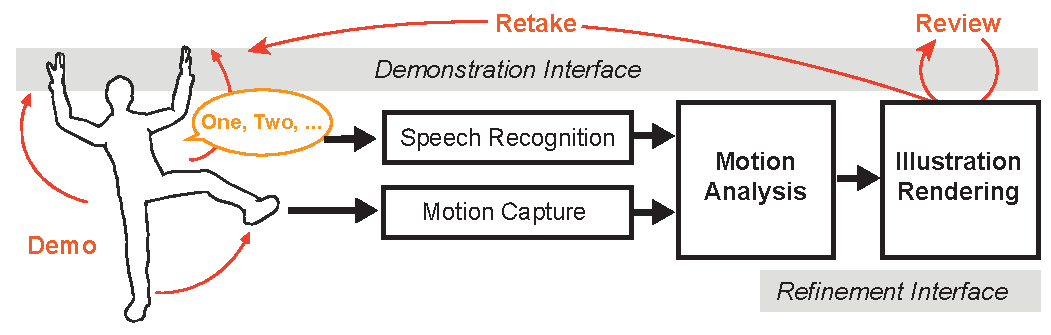
\includegraphics[width=0.8\columnwidth]{\democut/fig/pipeline}
  \caption{Given user markers, DemoCut analyzes both video and audio to segment the demonstration video and apply editing effects.}
  \label{fig:democut_pipeline}
\end{figure}

\begin{figure}[t]
  \centering
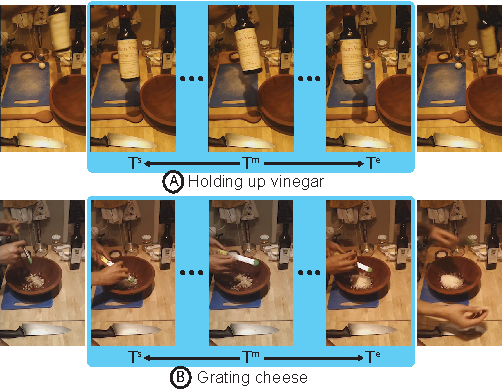
\includegraphics[width=0.6\columnwidth]{\democut/fig/video-similarity}
  \caption{DemoCut looks for similar video frames before and
after a marked frame $T^m$ to find candidate start ($T^s$) and end ($T^e$) frames
for the corresponding segment.}
 \label{fig:video-similarity}
\end{figure}

\subsection{Video Segmentation}

Except for the step marker, all of the user-specified markers indicate
important moments in the demonstration that correspond to some segment
of the recording. In many cases, we can infer the duration of these
segments by searching for video frames that look similar to the marked
frame. For example, in Figure~\ref{fig:video-similarity}A, the similar
frames before and after a supply marker show the author holding up a
bottle of vinegar, and in Figure~\ref{fig:video-similarity}B, the
similar frames around an action marker show the author grating cheese.
%
For every marked frame $T^m$, DemoCut uses the following method to
compute candidate start and end frames $T^s$ and $T^e$ for the
corresponding segment.
%
For the $i$-th marked frame $T_i^m$, our algorithm finds $T_i^s$ by
comparing $T_i^m$ to earlier frames in the video until it reaches a
previous marker at $T_{i-1}^m$, or until 5\% of pixels (in grayscale)
%in the grayscale versions of the frames
have changed by 20\%. Similarly, the system
finds $T_i^e$ by comparing $T_i^m$ to subsequent frames in the video.
To optimize performance, DemoCut compares to frames sampled at 0.5
seconds and ignores overlaps between segments. Segment overlaps are
resolved during boundary adjustment after incorporating the audio
analysis.

\subsection{Adjusting Segments with Audio Analysis}

Adjacent segments can have different effects that change how video and audio are processed. To prevent such changes from interfering with a video's narration, DemoCut adjusts segment boundaries to align with audio activity boundaries.
% DemoCut chooses different editing effects for different
% segments. Segment boundaries should therefore be carefully adjusted based on the audio
% track to avoid interrupting the author's narration.

\begin{figure}[t]
  \centering
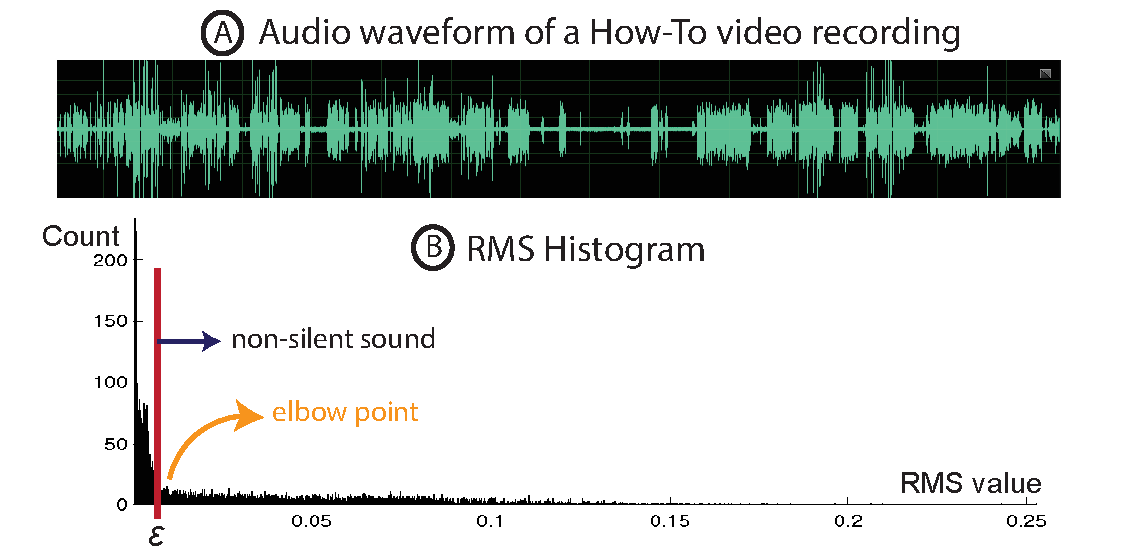
\includegraphics[width=0.8\columnwidth]{\democut/fig/audio}
  \caption{We use RMS energy of the audio to find silent and non-silent regions. We determine the threshold for silence by analyzing the histogram of the RMS energy.}
  \label{fig:audio}
\end{figure}

\subsubsection{Detecting non-silent sections}
%
Since many DIY videos include prominent non-speech sounds such as
chopping noises, power tools, etc., detecting speech automatically is
a challenging task. We found that even state-of-the-art speech
detection algorithms produce poor results in many cases.
%
As a result, we take a more conservative approach; DemoCut
automatically detects non-silent sections in the recorded
audio and treats the background sound as part of the narration.

At a high level, our algorithm for detecting non-silent sections works
as follows. We compute the ``loudness'' of each audio window,
organize the windows into a histogram based on loudness, and then
analyze the histogram to determine a minimum loudness threshold for
non-silent windows. We then apply this threshold to categorize all
audio windows as silent or non-silent. Finally, we filter this
categorization to eliminate very short sequences of silent or non-silent samples. Here, we describe these steps in more detail:
% \bh{I think we mean "window" instead of "sample" for the preceding section, since RMS operates on windows.}

\emph{Computing loudness.} Given an input audio waveform sampled at
44.1 kHz (Figure~\ref{fig:audio}A), we estimate loudness by computing
the root mean square (RMS) energy~\cite{Panagiotakis:2005eb} across
the entire waveform. The RMS energy
for a window of size $n$ is $\sqrt{(\sum_{n}{x_i^2})/n}$ where $x_i$ is the value of
the $i$th audio sample in the window. We set window sizes as 0.1 second with $n = 4410$. Prior to computing RMS energy, the audio is normalized and noise-reduced with Adobe Audition.

\emph{Computing loudness threshold.} After analyzing the RMS energy
profiles of several different types of DIY videos, we found that the
vast majority of recorded audio represents background sound, which
tends to have similar and fairly low RMS energy values. In contrast,
user narration varies from medium to high RMS values based on the
speaker's distance to the microphone and the sensitivity of the
recording device. Based on this observation, we first compute a histogram
of RMS energy for all windows in the audio track; the windows that
correspond to background sound form a large mass at the low-RMS end of
the histogram (Figure~\ref{fig:audio}B).
%
To distinguish these ``silent'' parts of the recording from the
narration, we smooth the histogram with a Gaussian kernel, find the
minimum derivative point in the smoothed histogram, and set the
loudness threshold $\varepsilon$ to be the RMS energy value at this
elbow point.
%
Figure~\ref{fig:audio}B shows the RMS histogram and loudness threshold
for one of our example videos, ``How to make salad dressing.''

\emph{Categorizing silent/non-silent sections.} To partition the audio
track into silent and non-silent sections, we first label each window
as silent or non-silent based on $\varepsilon$.
%
This initial labeling often includes some very short silent and
non-silent sections.
%
Since many short silent sections correspond to short pauses between
spoken words, we turn any silent sections that are shorter than 0.4
seconds into non-silent sections.
%
Then, we discard any non-silent sections that are shorter than 0.8
seconds to account for any clicks and pops in the recorded audio.
%
The 0.4 and 0.8 second thresholds for silent and non-silent sections
were tuned experimentally, and we used these parameter values for all
of our results.

\subsubsection{Adjusting segment boundaries}

In order to avoid cutting off an author's narration, DemoCut
adjusts the video segment boundaries using the non-silent sections
of the audio track (Figure~\ref{fig:democut_pipeline}). First, for any segment
%[$T_i^s$, $T_i^e$]
we find
all of the overlapping non-silent audio sections and then grow the
segment so that it completely contains all of these non-silent sections.
%
Next, DemoCut resolves overlapping segments: If any two segments
overlap,
%such that $T_{i}^{e} > T_{i+1}^{s}$,
the boundaries must be readjusted.
%
If the overlap region is silent, the region is split into two equal parts and each is assigned to the
corresponding segment.
%
If the overlap region includes a non-silent audio section,
DemoCut assigns this non-silent section to the segment that has
more overlap with the section. If the overlap for both video segments is the same, DemoCut assigns the section to the smaller video segment.
%
Finally, DemoCut addresses any gaps between segments. If a gap is less
than 2 seconds, it is merged to the shorter adjacent segment.
Otherwise, DemoCut creates a new segment for the gap. Note
that such {\em unmarked segments} do not have a corresponding marker, but
they may still show useful details of the demonstration.


%Using the non-silent sections of the audio track, DemoCut adjusts the video segment boundaries for each user-specified marker (Figure \ref{fig:audio}C). For a marker at $T_i^m$ with a shot boundary [$T_i^s$, $T_i^e$] where  $T_{i}^{s} > T_{i-1}^{e}$ and $ T_{i}^{e} < T_{i+1}^{s}$, we find all the overlapped non-silent sections during this time interval: {[$S_j^s$, $S_j^e$], [$S_{j+1}^s$, $S_{j+1}^e$], \ldots, [$S_{j+k}^s$, $S_{j+k}^e$]}.
%
%In order to have each video segment contains complete narration without a sound cutoff, we examine the first and last non-silent section and adjust the segment boundary to [$ min(T_{i}^{s}, S_{j}^{s}), max(T_{i}^{e}, S_{j+k}^{e}) $].
% Note: avoid sound cutoff if a segment is "skipped"

%After all the annotated segments are adjusted, for any two consecutive segments where their boundaries are overlapped that $T_{i}^{e} > T_{i+1}^{s}$ by $x$ seconds, if they share one speech section [$S_j^s$, $S_j^e$], assign this speech section to the video segment that overlaps more and adjust the start and end frames, i.e. either $T_{i}^{e'} = S_{j}^{e}$ or $T_{i+1}^{s'} = S_{j}^{s}$ so that $T_{i}^{e'} < T_{i+1}^{s'}$. If there is no speech section in the overlapped time frame, split into half, i.e. $T_{i}^{e'} = T_{i}^{e} + x/2$ and $T_{i+1}^{s'} = T_{i+1}^{s} - x/2$ (Figure \ref{fig:audio}D).

%In order to completely segment the entire recording, for any gap between annotated segments, if it falls below 2 seconds, merge to the shorter adjacent segment; otherwise, create an empty segment (Figure \ref{fig:audio}E).

\subsection{Applying Effects}

To automatically apply an effect to each
computed segment, DemoCut first detects whether
there is motion in the video. A segment is considered to be {\em static}
(i.e., no motion) if less than 1\% of pixels in the grayscale versions
of consecutive frames have changed by more than 20\%. To optimize for
performance, the segment is sampled at 0.5 seconds for this
comparison.
%
DemoCut chooses effects as follows:

\begin{enumerate}
  \item If the segment includes a \emph{cutout} marker, apply {\em ``Skip''}.
  \item If the segment includes a \emph{closeup} marker, apply {\em ``Zoom''} to the entire segment.
  \item If the segment includes any non-silent audio sections, apply {\em ``Fast Motion''}.
  \item If the segment is silent, static, and unmarked, apply {\em ``Skip''}.
  \item If the segment is silent but not static (either marked or unmarked), apply {\em ``Normal''}.
  \item For any marker with a text annotation, apply {\em ``Subtitles''}.

  \end{enumerate}
% \bh{Missing discussion of how to apply zoom and subtitles here. I think zoom is applied to the whole shot, while there are two levels of subtitles - one for the step level, and one for a shot/segment level.}

%These rules result in a default set of editing effects for the entire
%video tutorial. The information is saved as metadata to playback in the Editing UI. As described in the previous section, users can manually change the editing effect for any segment.

%!TEX root = ../thesis.tex
\subsection{Implementation}
The video and audio analysis is implemented in Matlab. The Annotation and Editing Interfaces are implemented with standard Web technologies (HTML5, CSS3, and JavaScript). An Apache web server hosts these web pages and sends the user annotations to the back-end Matlab system.
%Once the video is processed, the server updates the video rendered with generated metadata on the web interface. When user modified the automatic effects and text annotation in real-time, DemoCut records the changes and updates the metadata for outputs.

%!TEX root = ../thesis.tex
\section{Evaluation}

\begin{figure}[t]
  \centering
  \includegraphics[width=\columnwidth]{\democut/fig/results-small}
  \caption{Illustrative frames from the seven videos used to assess DemoCut. Labels correspond to task labels in Table~\ref{tab:system_results}.}
  \label{fig:results}
  \vspace{-0.2in}
\end{figure}

\subsection{Evaluating Automatic Effect Decision}

To evaluate DemoCut's analysis engine, we recorded seven how-to tasks
from the five categories we selected in the formative user study
(Table~\ref{tab:system_results}).
%
The tasks were recorded by 4 people (all authors of this
paper) in 7 locations using a Sony camcorder or an iPad with
a video resolution of at least 640x480 pixels.
%
We used DemoCut to annotate the recordings and then examined the
automatically generated tutorials.

Overall, the resulting tutorials exhibit many of the desired
characteristics outlined earlier in the paper.
%
The automatically edited videos are concise: 2-5 minutes long and 2.5
times shorter than the original footage.
%
In most cases, DemoCut successfully identified segments where the ``Fast
Motion'' or ``Skip'' effects could be applied to condense the tutorial.
%
For example, the edited salad dressing video uses ``Fast Motion'' to
speed up repetitive actions like chopping an onion and grating cheese,
and then skips the segment where the author leaves the frame to toast
pine nuts.
%
In addition, the automatically generated titles improve the clarity of
the tutorials by adding valuable descriptions of steps, actions,
supplies and indicating the elapsed time for skipped segments.
%
In an electronics tutorial, titles like ``sending data toggles LED''
add important details that are not visible in the video.

There were some situations where the effects were not as successful.
%
To get a more quantitative measure of DemoCut's performance, we
counted several types of errors in the automatically generated
videos:

{\em Incorrect editing effects.} In a few cases, the ``Fast Motion''
effect is applied to segments where the audio track should actually be
in sync with the visuals. Also, when markers are very close to one
another in time, DemoCut sometimes generates very short segments where the editing effects are hard to see.
%
We identify these cases as incorrect editing effects.

{\em Audio miss.} We refer to any piece of narration that is not
detected as a non-silent section as a miss.

{\em Audio cut-off.} We refer to any detected non-silent section that
cuts off narration by ending too early or starting too late as a
cut-off error.

{\em Audio false-positive.} We refer to any non-silent section that is
neither narration nor significant activity or background sound as a false-positive.

We report the incorrect edits as a percentage of the total number of
segments and the three audio errors as a percentage of the total
number of ground-truth narration sections.
%
Table~\ref{tab:system_results} shows all of the results from our
analysis.
%
Overall, we found low average error rates (less than 11\%) for all of
these problems.
%
Also, note that most of these errors can be fixed by changing the
automatically applied editing effects in DemoCut's reviewing and
editing interface.


%!TEX root = ../thesis.tex
\section{Evaluation}
\label{kinectograph_study}

This section presents user feedback collected from three preliminary studies that we conducted to answer questions: What activities would users find useful to capture using Kinectograph? How well could users create self-directed tutorials with Kinectograph?

\subsection{Study 1: Demo at an Expo}
We demonstrated an initial design of Kinectograph (see Appendix C) at a public exhibition to approximately 60 people. Each participant was allowed to enter our capturing space and experience the device. Based on our observation and conversations collected, we found that people were convinced by the idea as soon as they walked into the scene when Kinectograph started to move along. These questions were often asked: \iquote{How fast was Kinectograph able to follow me?} and \iquote{Can I switch to track other parts (like my hand)?}. With the tablet device control, participants soon were successful in controlling the camera. They often walked, ran, and danced to test the tracking. We also learned that people expected the device to provide fast response in various conditions such as turning, rapid change of directions, or partial occlusions (when people were hidden by furniture or large objects).

\subsection{Study 2: Test on Recording Activities}
To understand how Kinectograph can support users in demonstrations, we invited four participants (3 male and 1 female, aged 22-29) who did not join the exhibition to our user study in a home environment. We aimed to explore whether users prefer to watch the video captured by Kinectograph over video recorded with a static camera, and whether Kinectograph can capture complete demonstrations
 that a static camera cannot achieve.

We first introduced Kinectograph by having participants walk around while the device tracked. We encouraged participants to brainstorm some activities they wanted to record. Once the task was decided, they were asked to set up both a static camera and the Kinectograph with our tablet device and start the recording. There was no time constraint during the study. A short post interview was then conducted, in which we showed the recorded videos from both cameras on a PC.

\begin{table}[b!]
     \centering
    \includegraphics[width=1\columnwidth]{\kinectograph/fig/study2}
    \caption{Task information and results collected in the preliminary user study.}
    \label{tab:kinectograph_first_tasks}
 \end{table}

\begin{figure}[t!]
     \centering
    \includegraphics[width=0.5\columnwidth]{\kinectograph/fig/OurExamples-2x2}
    \caption{Examples of camera views captured by a static camera and Kinectograph at two specific moments in time.}
    \label{fig:kinectograph_dance}
\end{figure}

Table~\ref{tab:kinectograph_first_tasks} shows details of the four tasks and analysis of the recorded videos. We categorized physical activities into three movement types: \emph{Continuous} (user continuously moves around), \emph{Periodic} (user moves, stays, and moves again periodically), and \emph{Occasional} (no clear motion pattern was observed).
%
There were two Continuous and two Periodic tasks that participants designed. The moving range was about 15 feet in a home environment, and participants set the static camera about 8 feet away from the center of their workspace. Participants chose this distance to avoid out-of-frame problems with the static camera: \iquote{The distance was chosen so that all of the activity could be captured} (P4). Kinectograph was placed 6 feet away on a tabletop by the experimenters to capture the participant's whole body. Participants were allowed to adjust the camera angle via our tablet UI before recording the demonstration.

All the participants chose to track their heads, but note
that their activities involved frequent turning where
pure face recognition might fail. Participants did not
change this setting during the performance, although
they were allowed to. P2 changed to the manual mode
for testing, switched back, and then continued the
activity. The average video length is one and half
minutes long.

All the participants agreed or strongly agreed that
Kinectograph captured what they intended to show,
while only half of them agreed that the static camera
captured as expected. The main reason was the
limited static camera angle; in three tasks, participants
moved out of the static camera view more than once
. Figure~\ref{fig:kinectograph_dance} shows two examples where our system
captured what the static camera missed. It was worth
noting that although P3 had set and confirmed the
viewpoint before recording, he was not aware that he
shortly but frequently (9 times) went over the
boundaries when he was demonstrating. He explained
that he preferred using Kinectograph because it \iquote{kept
us in the center of view no matter how we moved
around.} This shows that Kinectograph successfully
ensured the activities would be captured and therefore
enabled users to focus on their tasks.

\subsection{Study 3: Self-Recording Activities}

Finally, we conducted a study to measure whether users could film an entire demonstration video using Kinectograph with minimal aid.
%
We recruited seven participants (3 male and 4 females, ages 20-33) from a university to record multi-step tutorials in a lab environment. Four had filmed a video before but only one had filmed a video without the assistance of others. Each participant was compensated with a \$10 giftcard. Each session lasted about 30 minutes long.
% Note that this experiment was run using a previous prototype of the Kinectograph base, which did not utilize the motors provided by the Kubi.
%\pc{describe the settings and put the figure here}
%14-16 feet by 12-14 feet area

\subsubsection{Procedure and Tasks}
\subsubTitleBold{Introduction (5 minutes)} Participants first went through an online documentation to learn the Kinectograph features. %with a demo video

\subsubTitleBold{Training (10 minutes)} Experimenters guided participants through a series of interactions highlighting each of our core features. Participants were asked to operate each feature through our Tablet UI with the support of experimenters.

\subsubTitleBold{Testing (5 minutes)} We asked participants to film a basketball tutorial using Kinectograph. They were asked to introduce actions including passing, catching, and tossing a basketball. Participants acted as both an actor and a director, i.e., they fully controlled the camera and performed the demonstrations without any assistance. A series of nine subtasks were designed for participants to exercise the following features: manual mode (pan/tilt), tracking mode (to track single and multiple body joints), and zooming. In particular, one of the subtasks involved two users in the view. Experimenter walked in the view for passing the ball when participant invited. To help participants understand these activities, we provided a storyboard with high level instructions for filming (e.g., ``zoom into your face'', ``pan to the basketball'', or ``track your head and walk around'') without explicitly listing which Kinectograph feature to use. During the recording, we captured Kinectograph's rendered video view.

\subsubTitleBold{Questionnaire and Debrief (10 minutes)} Finally, we asked participants to watch the recorded video in full and answer a questionnaire, regarding the ease of use of our interface and open-ended questions. We monitored the number of attempts it took to complete each filming task of the tutorials.

\subsubsection{Results}
% \subsubsection{Successes}
All of the 7 participants successfully created a self-directed tutorial using our system. No users failed to complete any of the 9 subtasks. Each participant reattempted at most 2 subtasks, mostly to reselect a zoom area. The average video length was 3.5 minutes. Overall, participants rated the ease of use of the system as $\mu=4.1$ on the 5-point Likert scale.
%
All participants were able to manually pan and tilt the camera by swiping as intended. Participants stated that this was easy to control with the UI ($\mu=3.6$ , $\sigma = 1.0$). They also successfully enabled the tracking mode and had Kinectograph track their head and hands. Participants stated it was easy to enable tracking ($\mu=4, \sigma=1.3$ ) and rated their satisfaction with the system performance as $\mu=4, \sigma=0.8$.  Participants stated that \iquote{It was easy to select a body part of choice} (P6), and that \iquote{ (...Kinectograph) could center the screen very well, and accurately tracked the person} (P7). Four users specifically mentioned that zooming was one of the features that worked well. Participants were satisfied with their video recording ($\mu=4.1$, $\sigma=0.7$).

%{\bf Reset} All participants were able to complete the reset task in one try. unimportant

% \subsubsection{Shortcomings}
We also learned some important shortcomings from the study. Notably, the pan-tilt motors that our previous Kinectograph prototype uses is under-dimensioned, which leads to oscillation (camera shake) when Kinectograph performs large amplitude pan movements. This is less noticeable at further distances, but becomes especially problematic when the users zooms in on small regions. Learning this effect, we have removed this issue with our current use of Kubi's servos, which provide smooth motor control.

Latency in video streaming to the tablet device hampered usability. As P4 stated: \iquote{The lag made it difficult for me to move the kinectograph smoothly [during manual control]}.
%
% Tracking multiple actors remained somewhat difficult (a confederate joined for a ball passing task). P1 stated \iquote{Shortcomings were only really with multiple people in the demo, and the limitations of the viewing angle of the Kinect itself.}
%
Participants also suggested alternative control modes other than a tablet while engaged in bi-manual tasks: \iquote{Certain demos require the use of multiple hands, meaning that I can't carry the iPad during the demo if i wanted to change the point of focus on my body. It would be nice if there were gestures i could do to switch the point(s) of focus without having to use the iPad.} We found this concept interesting and plan to explore in future work.

% \begin{figure}[t]
% \centering
% \includegraphics[width=1.0\columnwidth]{userStudy}
% \caption{We presented participants in the second procedure with a storyboard of actions they should perform.}
% \label{fig:storyboard}
% \end{figure}
% In aggregate, our evaluation suggests that Kinectograph system is capable of being used to create tutorial videos but also points the way for future work. Future work comprises improvements to live video streaming, better support of multiple users (i.e. using voice commands or gesture cues to control), and using kinectic info and zoom as meta data for playback. \dc{add more?}


% and more Tablet UI features, such as picture in picture view and more boxes on the UI to provide further feedback to the user.

%!TEX root = ../thesis.tex
\subsection{Results}

We gathered nine different tutorials and recorded working through each tutorial in Photoshop. We then used MixT to automatically generate mixed media tutorials from these demonstrations. This section describes this corpus. The following section then evaluates the generated tutorials quantitatively and qualitatively.

Our tutorials came from both online and book sources: two from \"Adobe Photoshop CS5 Classroom in a Book,\" five from photoshopstar.com, one from makeuseof.com, and one from icanbecreative.com. All are popular resources for Photoshop learners. Two of the tutorials were also used in the formative user study. The selected tutorials had a total of 165 steps and covered all five command types: they contained 15 brushing/drawing operations, 14 control point manipulations, 30 parameter adjustments, 67 UI navigations, and 39 layer operations. The demonstrations were recorded on three different laptops running Photoshop in full screen with native resolutions of 1680x1050, 1440x900, and 1280x800 pixels.

Overall, the MixT tutorials that we generated exhibit the desired characteristics that we identified in our formative study: scannable steps, small but legible videos, visualized mouse operations, and user control over presentation format. We highlight some interesting results generated by MixT and also refer readers to the provided video figure, which has additional examples.

Scannability: The step-by-step layout of our tutorials makes them easy to scan. For example, at a glance, we see that the tutorial \"Turning an Image into an Old Photo\" involves several adjustment layer operations, while the tutorial \"Creating Artistic Effects\" involves more parameter adjustments and brushing commands.

Mouse visualization: Our mouse visualizations help clarify several interactions. They clearly communicate the difference between clicking and dragging, a distinction that is fundamental to operations such as path manipulation but hard to glean from screen capture video. For example, Figure~\ref{fig:mixt_results}A shows the difference between moving around the contour of an object without drawing a path (left), and dragging a Bézier handle to adjust a path segment (right). Mouse trails and click markers were also useful for showing the trajectory of lasso selections (Figure~\ref{fig:mixt_results}B).

Zoom and crop modes: For many steps, the zoom and crop videos offer clear legibility benefits over the normal video mode. In our corpus, zoom mode was especially valuable for highlighting actions on small buttons that occurred near the frame boundaries, e.g., in the layers palette (Figure~\ref{fig:mixt_results}C right). Such operations are easy to miss in a normal, scaled video (Figure~\ref{fig:mixt_results}C left). Crop mode was useful in showing the effect that parameter selection has on the canvas. Figure~\ref{fig:mixt_results}D shows two successive frames that illustrate how changing a layer's blending mode affects the image. Enlarging the canvas in these modes also helps users see the details of effects, such as applying the eraser tool on the canvas to enhance the underlying layer (Figure~\ref{fig:mixt_mouse}).

\begin{figure*}[t]
  \centering
  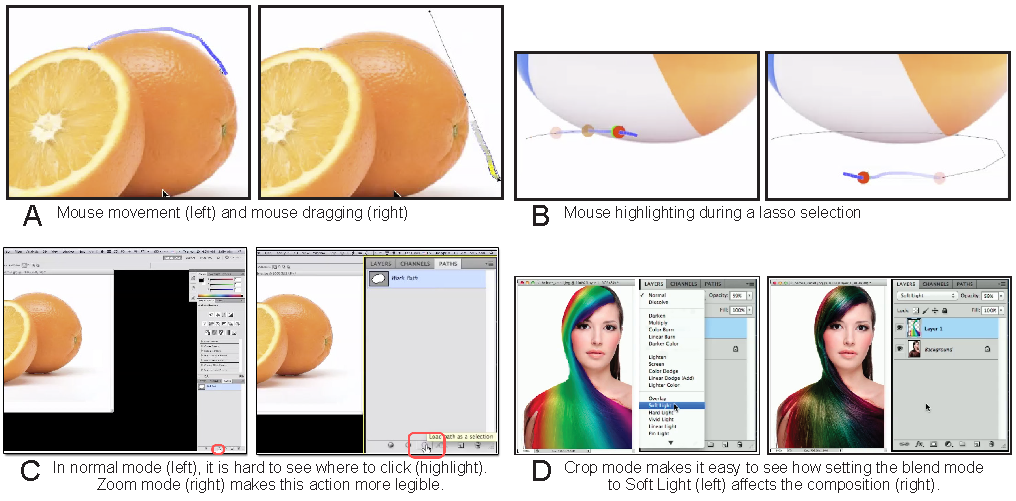
\includegraphics[width=\textwidth]{\mixt/fig/mixt_results/mixt_results}
  \caption{Automatically-generated MixT results.}
  \label{fig:mixt_results}
\end{figure*}

%!TEX root = ../thesis.tex
\section{Conclusion}

In this paper, we presented DemoCut, a semi-automatic video editing
system that helps users create clear and concise video tutorials of
DIY tasks. The key idea behind our approach is to combine rough user
annotations with simple video and audio analysis techniques in order
to segment the input recording and apply appropriate editing
effects. Our small user evaluation suggests that video authors are
able to create effective video tutorials using DemoCut, and the
qualitative feedback includes encouraging positive reactions to the
annotation and editing workflow, as well as the automatic editing
effects.

% \section{Limitations and Future Work}

Our implementation is based on several simplifying assumptions that
limit generality. We assume a single, static camera position that
shows all relevant actions and a quiet indoor environment with
constant lighting and little background noise. In order to detect static shots  that should be skipped, our video analysis assumes a static background. Our audio analysis assumes that all non-silent sections of audio are narration, but this may not always be the case. Loud non-speech sounds, such as chopping or the sound of a sewing machine, can lead to errors in our editing effect decisions.

As was pointed out by several of our study participants, making effect decisions individually for each segment can lead to inconsistencies in playback speed as the video transitions from segment to segment. A more global approach that looks at all video effects together and enforces  smooth transitions between adjacent segments would help address some of these artifacts.
%
In addition to addressing these limitations, we see several promising
directions for future work.

\subsubTitleBold{Multiple camera footage.} We designed DemoCut to work with
footage from a single, static camera. One interesting avenue for
future work is to consider footage from multiple cameras. Prior work has compared different camera views capturing physical
tasks for remote collaboration \cite{Fussell:2003te,Ranjan:2007}. Similarly, DemoCut could try to automatically select the best view for
each segment based on user annotations as well as the video content
(e.g., choosing a zoomed view for closeups, switching to a
different view when there are occlusions). % \bh{cite Ranjan here?}

\subsubTitleBold{Support viewer's learning.} In this work, we focus on producing
well-edited video tutorials. However, we could also imagine generating
different output formats, including indexed
videos, step-by-step instructions, or mixed media tutorials, similar
to those presented by Chi et al.~\cite{Chi:2012fq}. Another natural extension would
be to develop interactive components that monitor user actions and
provide realtime guidance and feedback for general DIY tasks. Follow-up studies to understand viewer's learning experience would be useful for refining the automatic editing effects and interactive design.
% Different output formats and understand viewer's perspective.
% {\bf Interactive DIY tutorials.} Recent work has demonstrated
% interactive tutorial systems that help users follow specific types of
% physical tasks, such as assembling Duplo models~\cite{Gupta:2012ku}.
% A natural extension of our work would
% be to develop interactive components that monitor user actions and
% provide realtime guidance and feedback for general DIY tasks.

\subsubTitleBold{Generalize to other instructional video domains.} One exciting direction is to explore other areas where our techniques could be applied, such as software learning, music instruction, and video lectures. Each domain may require slightly different analysis and segmentation rules. For example, the system could use a log of executed operations to adjust segment boundaries for software tutorials, or incorporate pitch detection when analyzing music instruction.

% \section{Acknowledgments}

% Work at Berkeley was supported by Adobe and a Berkeley Fellowship for Graduate Studies.
% %
% We thank the YouTube users (in alphabetical order) \textit{donyboy73, Griffin Hammond on Indy Mogul, John NYCCNC, Matt Richardson on MAKE, mjfpieters, and TheMuskokaPainter} for sharing their insights on DIY tutorials in our interviews.

%\bh{still need to fix widows and orphans throughout.}

